\documentclass[11pt, a4paper]{article}
\usepackage[nochapters]{classicthesis}                              % template
\usepackage[margin=42mm]{geometry}                                  % margins
\usepackage[utf8]{inputenc}                                         % allow utf-8 input
\usepackage[T1]{fontenc}                                            % use 8-bit T1 fonts
\usepackage{graphicx}                                               % images
\usepackage{url}                                                    % URL typesetting
\usepackage{booktabs}                                               % good-looking tables
\usepackage{multirow}                                               % for tables
\usepackage{amsfonts}                                               % blackboard math symbols
\usepackage{amsmath}                                                % math ops
\usepackage{nicefrac}                                               % compact 1/2, etc.
\usepackage{microtype}                                              % microtypography
\usepackage{float} %to force figures to appear at a specific location

\definecolor{darkblue}{rgb}{0, 0, 0.5}                              % define link color
\hypersetup{colorlinks=true,citecolor=darkblue,                     % set link color
            linkcolor=darkblue, urlcolor=darkblue}

% Your packages here
% \usepackage{...}                                                  % some info, maybe

% !!! PLEASE CHANGE THESE VARIABLES TO MATCH YOUR INFORMATION !!!

\def\thesistitle{The Main Title of the Thesis}                      % title
\def\subtitle{The Subtitle of the Thesis If It Has One}             % subtitle
    % ^if there is no subtitle, replace by \def\subtitle{}  
\def\yourname{Your Name}                                                                       % ^first and last nam
 \def\yourprogramme{Cognitive Science \& Artificial Intelligence}    % uncomment this
\def\yourstudentnumber{000000}                                      % ANR (or u-number)
\def\finalmonth{January}
\def\finalyear{2000}
\def\supervisor{dr. Your Main Supervisor}
\def\committee{prof. dr. The Second Reader}
\def\acknowledgments{Some room for acknowledgements.}
\def\wordcount{your word count should be here, ex 12000}
% METADATA

\hypersetup{pdfauthor   = \yourname,
            pdftitle    = \thesistitle\ \subtitle,
            pdfsubject  = \yourprogramme\ Master Thesis
}

% CHOOSE EITHER OF -----------------------------------------
% IEEE STYLE:

% \usepackage[square,numbers]{natbib}                               % bracket-style refs
% \usepackage{natbib}                                               % OR: parenthesized refs
% \bibliographystyle{IEEEtranN}

% OR -------------------

\usepackage[natbibapa]{apacite}                                     % only parentheses
\bibliographystyle{apacite}                                         % 'cause APA

% !!! ------------------------------------------------------ !!!

\begin{document}
\input{frontmatter.tex}  % don't remove this :)

% --- start writing below:

\begin{abstract}
This is where the abstract goes. Don't forget to change the variables in \texttt{main.tex} to change all general placeholders shown in this document. The \texttt{frontmatter.tex} file should be left alone. The abstract should summarize in 150-250 words the contents of the thesis, mentioning: 1) the research goal, 2) the methods employed, 3) data collected or dataset/s used, 4) the main findings.
\end{abstract}

\section{Data Source, Ethics, Code, and Technology statement}
Checklist for creating a Data Source, Ethics, Code, and Technology (DSECT) statement:
Please provide answers to all below questions for transparency purposes when writing your ethical statement. There is no one-fits-all solution to ethical statements, and they heavily
depend on the nature of the study. After the questions below, an example DSECT statement is provided. 
\begin{itemize}
    \item[•] {Data Source}
    \begin{itemize}
        \item[o] {Who is the owner of the data?}
        \item[o] {Does the thesis project involve collecting data from human participants or animals?}
        \item[o] {Does the owner of the data give consent?}
        \item[o] {How and through what channel is the data acquired?}
    \end{itemize}
    \item[•] {Figures}
    \begin{itemize}
        \item[o] {Did you create all the images and figures?}
        \item[o] {Do you have consent for the images that you did not generate?}
    \end{itemize}
    \item[•] {Code}
    \begin{itemize}
        \item[o] {Did you use parts of the code from another study/someone else?}
        \item[o] {Did you list, including version number, all libraries and frameworks used?}
    \end{itemize}
    \item[•] {Technology}
    \begin{itemize}
        \item[o] {Did you use any tools or services to paraphrase the given text (for example a thesaurus or the Academic Phrasebank)? Please name them.}
        \item[o] {Did you use any tools or services to check spelling or grammar? Please name them.}
        \item[o] {Did you use any tools or service to typeset the given text? Please name them.}
        \item[o] {Did you use any reference management software other than the latex template? If so, please name it.}
        \item[o] {The following \textbf{statement should be included}: During the preparation of this work, the author used [NAME TOOL / SERVICE] in order to [REASON]. After using this tool/service, the author reviewed and edited the content as needed and takes full responsibility for the content of the thesis.}
    \end{itemize}
\end{itemize}


A DSECT Statement can be generated by answering the questions listed above and excluding the questions when not applicable.\

\subsection{Source/Code/Ethics/Technology Statement Example} \label{subs:DESCT}
Data Source: 
The (DATA) has been acquired from the (DATA SOURCE) through an online request. The obtained data is anonymised. Work on this thesis did not involve collecting data from human participants or animals. The original owner of the data and code used in this thesis retains ownership of the data and code during and after the completion of this thesis. However, the institution was informed about the use of this data for this thesis and potential research publications.
All the figures but Figure A and B belong to the author. To use Figure A and Figure B, the author received written permission via an email from FIGURE OWNER (AFFILIATION). The thesis code can be accessed through the GitHub repository following the link [CODE LINK].
Part of the CODE has been adapted by the author from (SOURCE, licensed under a CC0 BY 4.0). The reused/adapted code fragments are clearly indicated in the notebook. In terms of writing, the author used assistance with the language of the paper. A generative language
model (MODEL NAME + SOURCE) was used to improve the author's original content, for paraphrasing, spell checking and grammar. No other typesetting tools or services were used.


\section{Introduction} \label{sec:introduction}

Here you write the introduction. Start with briefly describing the research domain, why the topic is relevant, and current state-of-the-art by referencing pertinent research articles. Then, state your specific research goals/questions (you can separate them as shown below), followed by a one-paragraph summary of your findings. Discuss how answering your research questions can produce scientific relevance (domain insights) and societal relevance (real-world applications and/or benefits). 

You can refer to chapters like the current Section~\ref{sec:introduction}. If you want to list research questions it's probably best to use \texttt{quote} and/or \texttt{itemize}, like so:

\begin{quote}
\emph{To what extent we define a main research question?}
\end{quote}

\noindent The sub-questions can be listed seperately, as such:

\begin{itemize}
    \item[RQ1] \emph{How does sub question one influence the main RQ?}
    \item[RQ2] \emph{To what degree does sub question add anything?}
\end{itemize}

\noindent Or, format it as you desire (tip: you can nest \texttt{itemize} as well). You can alternate \emph{emph} and \textbf{textbf} however you wish. This should cover most of the things required for the introduction.

\section{Related Work}

Here you provide a synthesis of the existing literature, comparing and drawing parallels across studies to establish the state-of-the-art. Cite relevant theories, models, and recent work. Describe what prior research has found, any contradicting findings or competing approaches. Identify any gaps or limitations in existing research and how your thesis potentially addresses these gaps in terms of methodology, data used, etc.

Copy paste BibTeX code\footnote{Using e.g. the quote icon in GScholar, then BibTeX at the bottom.} and put it in \texttt{references.bib}. After, you can cite some work \citep{mackay2003information} -- using \texttt{\textbackslash citep}. You can refer to the author of e.g. \cite{minsky1961steps} directly like using \texttt{\textbackslash cite} (this does not work when using bracket-citation). If you use bracket-style,\footnote{Find the \texttt{natbib} part in the \texttt{main.tex} \LaTeX{} script.} you might want use \texttt{\textbackslash citeauthor} when citing, like: see \citeauthor{ananny2018seeing} \cite{ananny2018seeing}.  If you want to add pages you can use brackets in \texttt{\textbackslash citep[][p. 5]\{mackay2003information\}}, which looks like: \citep[][p. 5]{mackay2003information}. The first brackets can be used for things like \emph{see}, and \emph{e.g.}. If you want to cite multiple authors, simply comma-separate them (\texttt{\textbackslash citep\{\-minsky\-1961\-steps,\-mackay\-2003\-information\}}) and it will aggregate them automatically \citep{minsky1961steps,mackay2003information}.

\section{Methods}

\subsection{Dataset}
The CogPilot dataset (Rao,2022) was used in this project and are publicly available via PhysioNet (Goldbeger,2000). In the original experiment, volunteers performed virtual flight landing tasks over 4 difficulties. They had to mainly use cockpit instrument readings to follow an ideal path to land the aircraft inside a virtual reality setting. Each participant performed 12 runs divided evenly into 3 groups with each run under one difficulty level. Multiple wearable sensors were used to collect multimodal physiological data during the experiment. Table 1 gives an overview of sensor data and sampling rate. Flight performance was calculated as vertical and horizontal deviation from ideal landing path, and difference of ideal airspeed. table 2 shows detailed difficulty levels setup.  

For machine learning studies, the sub-sections may include: \textbf{Dataset/s} (i.e., source, size, features, and descriptive statistics where appropriate), \textbf{Feature Extraction} (if applicable), \textbf{Machine Learning Setup} (i.e., dataset splits, cross-validation approach, preprocessing steps, algorithms used, hyperparameters tuned), \textbf{Evaluation Metrics} (i.e., how model performance was assessed), \textbf{Implementation} (i.e., programming languages, packages used). 

If you define any equations (\verb|\begin{equation}...|), you probably might want to define everything using math operators (e.g., \verb|$D$|) and cite the work (!). So for example, following \cite{lewis1994sequential}, representing a document $d \in D$ as tf$(d)$, we define a probabilistic model $(d | Y = y)$ for all documents in class $y$, and select $y$ most likely to generate $d$:

\begin{equation} \label{eq:nbarg}
    \hat{y} = \underset{y}{\mathrm{argmax}} \ P(d | y) \cdot P(y)
\end{equation}

\begin{figure}[H] %forces the figure to appear here
    \centering
    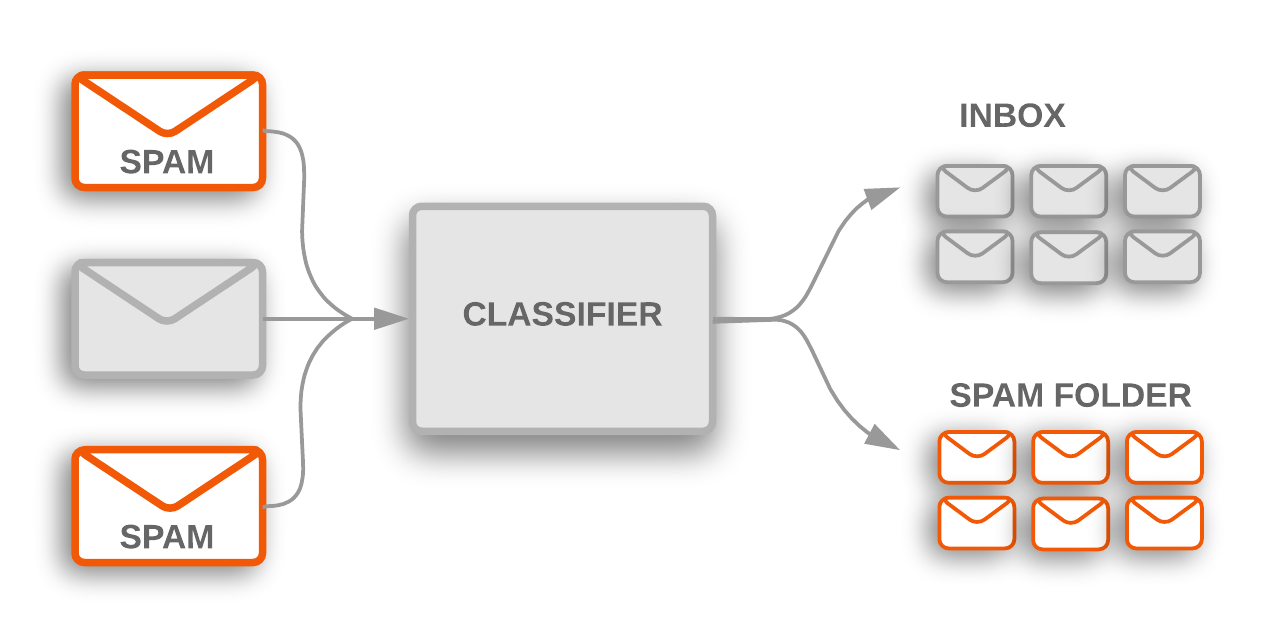
\includegraphics[width=\textwidth]{spam.png}
    \caption{Spam classification example. Source: \href{https://developers.google.com/machine-learning/guides/text-classification}{Google} (CC BY 4.0).}
    \label{fig:spam}
\end{figure}

With this we can detect spam (see Figure~\ref{fig:spam}) or bots.  Note that the figures (and tables for that matter) might not always be placed in this section. \LaTeX{} typically determines where to best put your objects. However, the [H] option from the float package forces figures to appear at this exact location rather than floating to other sections. \textbf{NOTE}: this Figure has a Creative Commons license; you cannot re-use other authors' figures without explicit permission or permissive licensing (as this would mean copyright infringement). You can refer to the equations as well (Equation~\ref{eq:nbarg}).

\section{Results}

Report your main findings here (e.g., model performance metrics, statistical test outcomes) and highlight important or interesting patterns. All information in tables and figures should be summarized/interpreted in text focusing on notable trends and comparisons.
Where appropriate, conduct further exploration through statistical analysis, confusion matrices, error analysis, or stratified results (e.g., performance across sub-groups, classes, or conditions) to reveal patterns not obvious from overall results.

\textbf{Figures and tables}: Use high-quality visualizations with labeled axes, clear legends, and informative captions (see Figure~\ref{fig:probs}). For table formatting, see Table~\ref{tab:results} as an example. Highlight important scores with \verb|\textbf{}|, use booktabs commands for structure: \verb|\toprule \midrule \bottomrule|. APA does not allow vertical lines.

\begin{table}
    \caption{Best scoring models classifying bots on Twitter and Facebook, respectively. $F_1$ scores report positive (bot) class. Outline text left (l) and numbers right (r).}
    \label{tab:results}
    \centering
    \small
    \begin{tabular}{llrr}
        \toprule
                              &                                   & \multicolumn{2}{c}{$F_1$ score} \\
                                                                  \cmidrule{3-4}
        PCA                   &  Models                           &  Twitter        &  Facebook       \\ 
        \midrule
        \multirow{3}{*}{300}  & Linear SVM ($C = 0.1$)            &   0.51          & \textbf{0.91} \\
                              & Random Forest ($S = 5, F = 5$)    &   0.71          & 0.85 \\
                              & Naive Bayes                       &   0.61          & 0.73 \\
        \midrule
        \multirow{3}{*}{500}  & Linear SVM ($C = 0.1$)            &   0.55          & 0.84   \\
                              & Random Forest ($S = 5, F = 5$)    &   \textbf{0.76} & 0.71 \\
                              & Naive Bayes                       &   0.41          & 0.64 \\
        \midrule
                              & Majority                          &   0.50          & 0.60 \\
        \bottomrule
    \end{tabular}
\end{table}

\begin{figure}
  \centering
  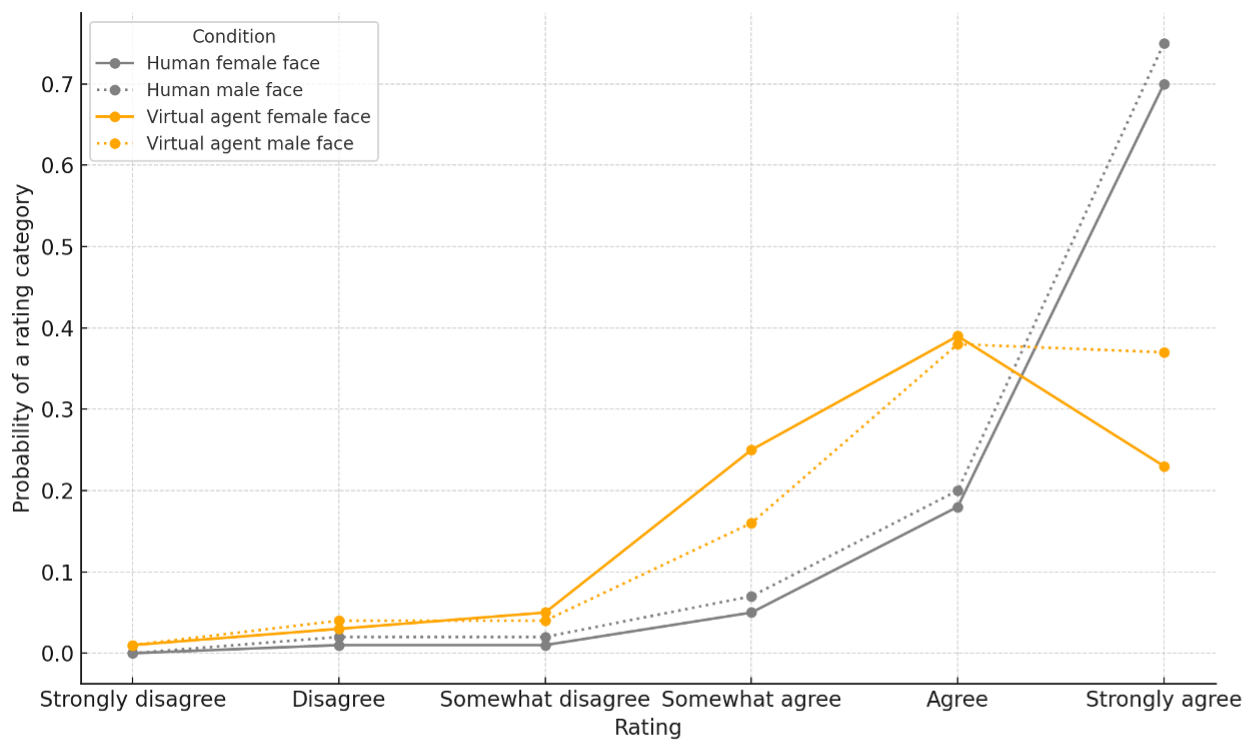
\includegraphics[width=\textwidth]{Example_plot.png}
  \caption{Cumulative probabilities based on Image Type (human and virtual agent) and Gender (female and male) for each outcome of a rating: from “Strongly disagree” to “Strongly agree”.} 
  \label{fig:probs}
\end{figure} 

\subsection{Some Model} \label{subs:model}

If you have anything specific to talk about, use subsections, and refer to them as Section~\ref{subs:model}. Don't use paragraphs or subsubsections.

\section{Discussion}

Here you interpret your findings in light of your research goals and the broader literature. Begin by briefly restating your research goal and summarizing your main findings. Then, discuss how these results relate to the existing research context established in your Introduction, i.e., do they confirm, contradict, or extend prior work? What is the specific contribution of your thesis?

Discuss your findings in the same order presented in the Results section. Offer interpretations for surprising or unexpected outcomes relying on the existing literature. Acknowledge any limitations of your methods, models, or data that may have affected your results, and explain how these limitations impact the validity and scope of your findings. Where relevant, suggest alternative approaches that could address these limitations.

Conclude by identifying directions for future research based on your findings, what questions remain unanswered? What new questions has your thesis raised?

\section{Conclusion}

Here you provide a concise summary of the overall work in your thesis. Essentially, you want to answer: what are the key takeaways? Clearly articulate the implications of your work: what does it mean for the field, for practice, or for theory?

Keep this section focused and avoid introducing new information, as that belongs in the Discussion.

\bibliography{references}

\section*{Appendix A} \label{app:a}

If you have nothing to append: remove this. You can do a page referral for these, like: Appendix A (page~\pageref{app:a}).

\section*{Appendix B}

And this!
\end{document}